\section{Rearranging Calculations}\label{sec:2}
The number of calculations is now split into $P = \num{100}$ and
$X = \num{100}$. In this case we get a value of
\begin{equation}
	\final = \num{3.15 \pm 0.16}.
\end{equation}
This value has a much smaller error (\per{5.1}) compared to \cref{sec:1}. A histogram 
for the distribution of $\pi_x$ is shown in \cref{fig:pi_hist_100_100}.
In that case the $\pi_x$ histogram resembles a gaussian distribution.\par
%
With $P=1$ and $X = \num{10000}$ we get a value of 
\begin{equation}
    \final = \num{3.2\pm 1.7},
\end{equation}
which is identical to the calculation from \cref{sec:1}. In fact, they have to be 
the same because they are mathematically the same. In the special case where 
$X = 1$, the final $\pi$ value is given by 
\[
	\final = \frac{4}{P}\sum_{p=1}^P\iv{r_p^2 \leq 1} \qquad 
	\Delta \final = \sqrt{\frac{1}{P-1}\sum_{p=1}^P(4\iv{r_p^2 \leq 1} - \final)^2}
\]
with using the definition of the variance from above. For the special case 
of $P = 1$ and the uncertainty from \cref{eq:pi_final} we get 
\[
	\final = \frac{4}{X}\sum_{x=1}^X \iv{r_x^2\leq 1} \qquad 
	\Delta \final = \sqrt{\frac{1}{X - 1}\sum_{x=1}^X (4\iv{r_x^2 \leq 1} - \final)^2}.
\]
For $X = P$ it is clear that they are the same, so similar results are expected. 
Since we can compare the results for both extreme cases, one can make the assumption that 
the definition of \cref{eq:uncertainty_for_one_x} for $X=1$ is as good as 
the definition in \ref{eq:pi_final} for the general case.\par 
Rearranging how we spent the random numbers makes a difference, because 
with using fewer experiments the uncertainty should get higher because there are 
fewer values that contribute to the uncertainty, but on the other hand 
the opposite will happen because the fewer $\pi_x$ values that we calculate will 
be more precise because they were calculated with a bigger number of generated points. 
This will be shown in \cref{sec:3}.


\begin{figure}[h!]
	\centering
	\begin{minipage}{0.45\linewidth}
		\centering
		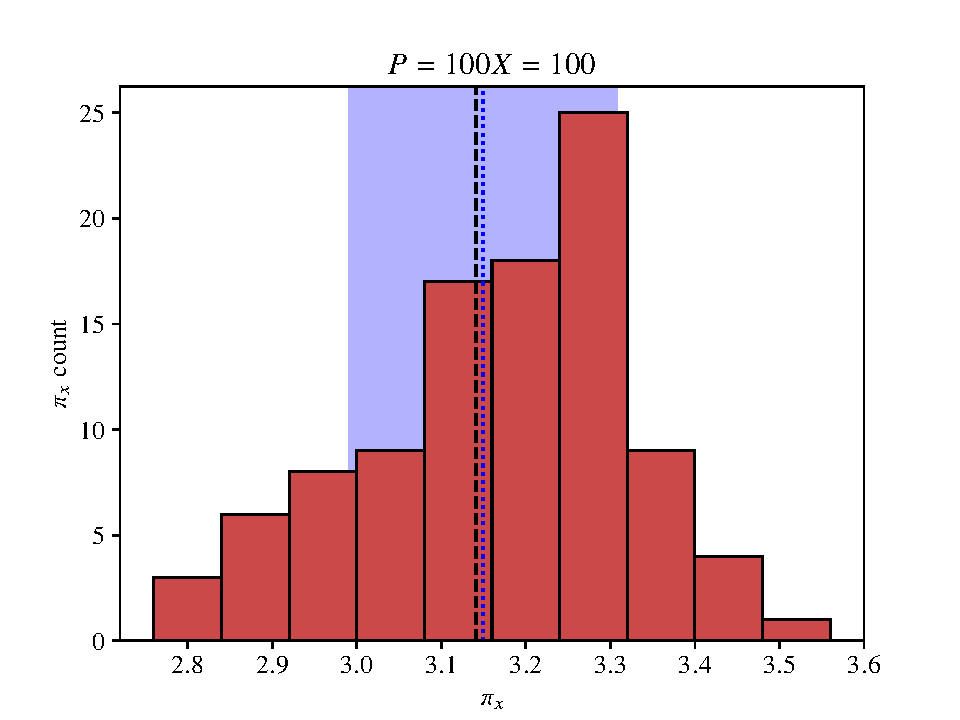
\includegraphics[width=\linewidth]{figs/ex1.2_pi_hist_100_100.pdf}
		\caption{Histogram of calculated $\pi$ values with $P = 100$ and
			$X = 100$.}
		\label{fig:pi_hist_100_100}
	\end{minipage}
    \hfill
    \begin{minipage}{.45\linewidth}
       \centering
       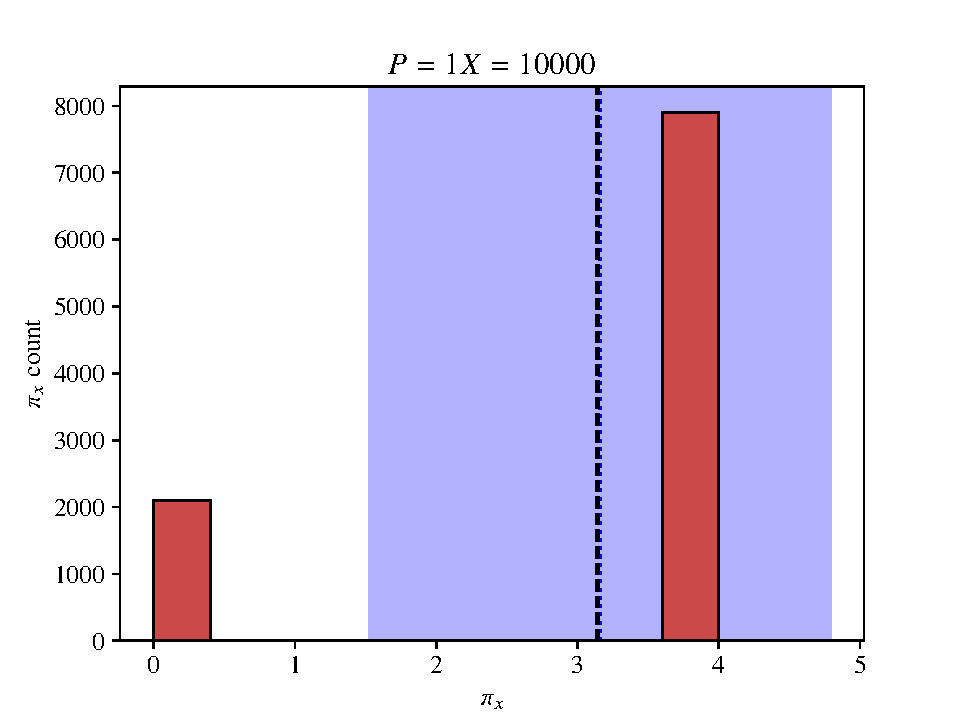
\includegraphics[width=\linewidth]{figs/ex1.2_pi_hist_1_10000.pdf} 
		\caption{Histogram of calculated $\pi$ values with $P = 1$ and
			$X = \num{10000}$.}
		\label{fig:pi_hist_1_10000}
    \end{minipage}
\end{figure}








